\documentclass[twocolumn]{article}
\usepackage[utf8]{inputenc}
\usepackage{graphicx}
\usepackage{tabularx}
\usepackage{subfigure}
\usepackage{hyperref}
\voffset = -100pt
\hoffset = -50pt
\headheight = 0pt
\textwidth = 550pt
\textheight = 750pt
\author{Name Surname }
\setlength{\columnsep}{0.3cm}
\usepackage{blindtext}
\pagestyle{empty}
\footskip = 0pt
\bibliographystyle{plain}

\begin{document}

\section*{Viktor Pavlov 230335TAF}
\section{Problem Statement}
In the domain of algorithmic music composition, different strategies can lead to a wide range of outputs in terms of quality and the style of the results. The goal of this study is to explore and compare the musical outputs of two types of models: Music Transformer~\cite{huang2018music} model and Recurrent Neural Network (RNN) models. The Music Transformer model extends the classic Transformer model with relative attention mechanism, which modulates attention based on how far apart two tokes are~\cite{shaw2018selfattention}. The relative self-attention mechanism allows the model to generate outputs with long-term coherence that extends beyond the length of the training examples. In comparison to the Transformer model, RNNs, including Melody RNN and Performance RNN~\cite{46748}, are simpler models that can be used to generate monophonic melodies and performance-like polyphonic sequences respectively.

\section{Music Transformer}
\begin{figure}[htbp]
  \centering
  \begin{minipage}[t]{0.45\columnwidth}
    \centering
    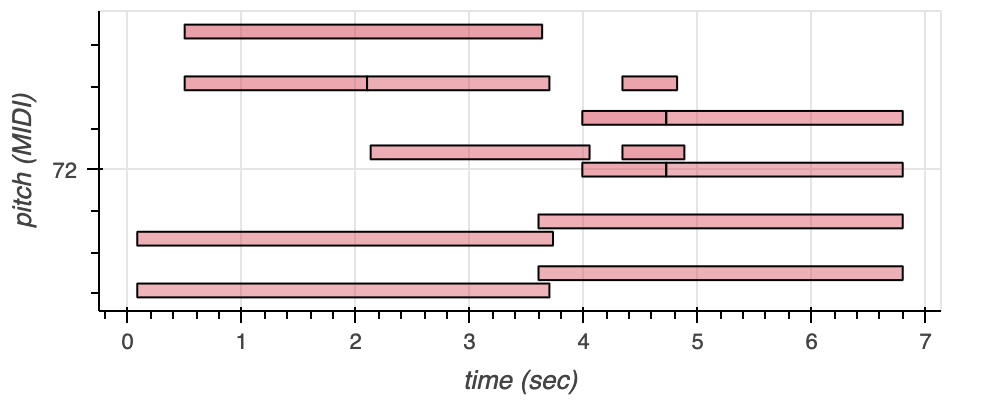
\includegraphics[width=\linewidth]{images/primer.png}
  \end{minipage}\hfill
  \begin{minipage}[t]{0.45\columnwidth}
    \centering
    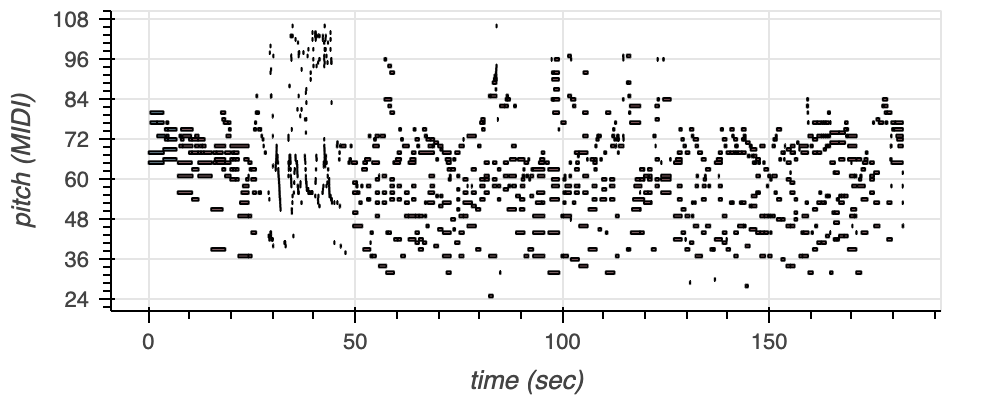
\includegraphics[width=\linewidth]{images/tf_continuation.png}
  \end{minipage}
  \caption{Continuation (right) generated by the Unconditional Transformer model based on primer (left).}
  \label{fig:groupedImages}
\end{figure}
In the course of this study, I utilized two Music Transformer models from Google's Magenta library~\cite{magenta}: Unconditional and Score Conditioned. The Unconditional model, although is capable of generating continuations from a given primer melody (as can be seen in Figure~\ref{fig:groupedImages}), can also generate music without an initial seed, relying on its understanding of musical patterns and structure. On the other hand, the Score Conditioned model works in a sequence-to-sequence manner by generating new interpretations of the provided score. This includes capabilities like generating new accompaniment for a given melody, similarly to adding a new dimension to the input (illustrated in Figure~\ref{fig:groupedImages2}). Both models were trained on the MAESTRO dataset~\cite{hawthorne2018enabling}. The MAESTRO (MIDI and Audio Edited for Synchronous TRacks and Organization) is a dataset composed of about 200 hours of virtuosic piano performances captured with fine alignment ($\sim3$ms) between note labels and audio waveforms. Additionally, the models use the score-to-performance (Score2Perf~\cite{score2perf}) encodings that enrich the MIDI~\cite{midi1996} grid-like representations of music with slight variations in timing and velocity in order to achieve a more human-like sound.

\begin{figure}[htbp]
  \centering
  \begin{minipage}[t]{0.45\columnwidth}
    \centering
    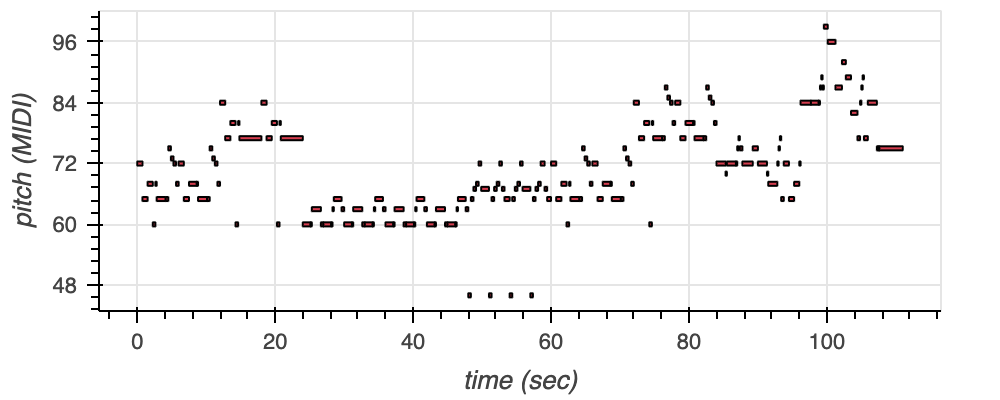
\includegraphics[width=\linewidth]{images/avril_melody.png}
  \end{minipage}\hfill
  \begin{minipage}[t]{0.45\columnwidth}
    \centering
    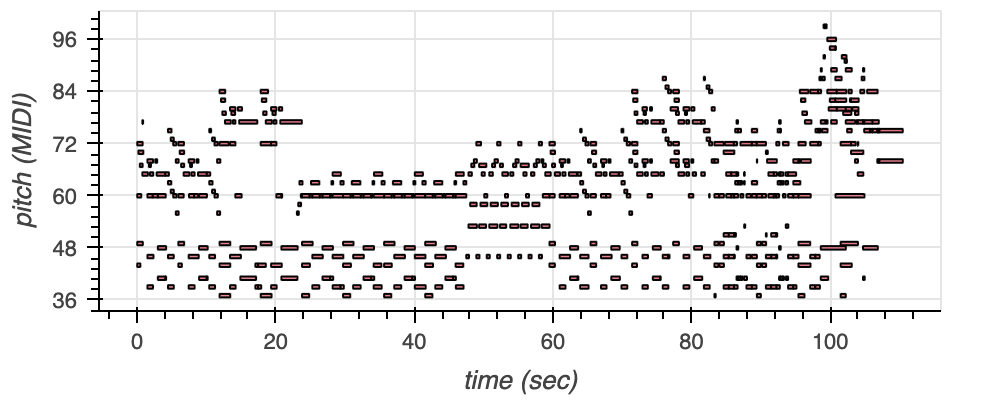
\includegraphics[width=\linewidth]{images/avril_acc.png}
  \end{minipage}
  \caption{Accompaniment (right) generated by the Score Conditioned Transformer model based on melody (left).}
  \label{fig:groupedImages2}
\end{figure}

\section{RNNs}
For comparison to the Transformer model, Recurrent Neural Network (RNN) models were utilized from the Magenta library: Melody RNN and Performance RNN. The Melody RNN is a model specifically designed to handle monophonic melodies, while the Performance RNN model is designed for polyphonic piano music with expressive timing and dynamic. Both models have a LSTM-based architecture and were trained on large dataset of MIDI files, allowing them to learn a wide range of musical styles and sturctures.

\section{Model Comparison}
\begin{figure}[htbp]
  \centering
  \begin{minipage}[t]{0.45\columnwidth}
    \centering
    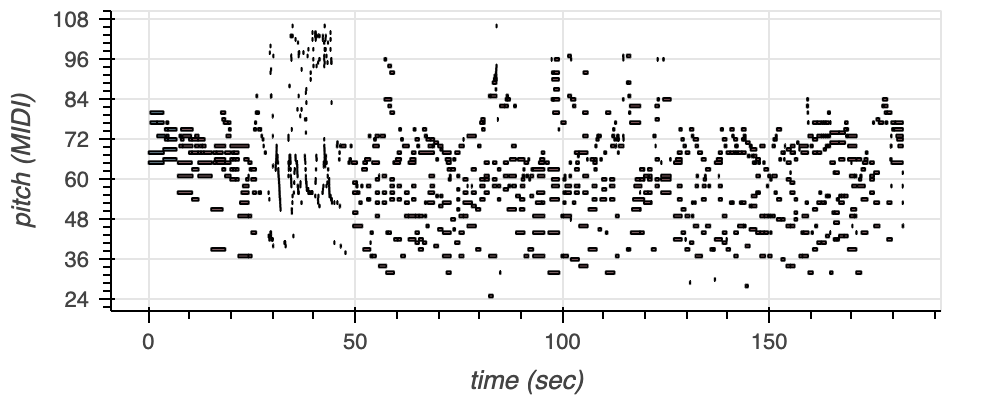
\includegraphics[width=\linewidth]{images/tf_continuation.png}
  \end{minipage}\hfill
  \begin{minipage}[t]{0.45\columnwidth}
    \centering
    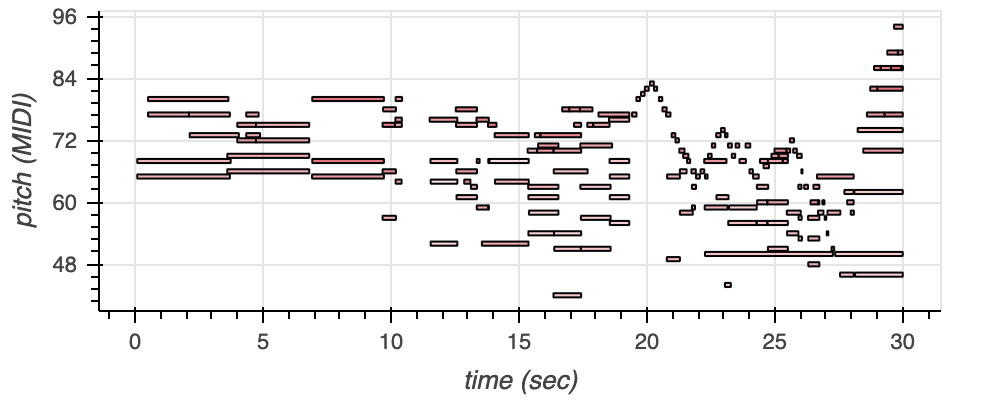
\includegraphics[width=\linewidth]{images/rnn_continuation.png}
  \end{minipage}
  \caption{Transformer continuation (left) and RNN continuation (right).}
  \label{fig:groupedImages3}
\end{figure}
In order to compare the models I used the following criteria: musical quality, efficiency and flexibility.
\paragraph{Musical Quality}  The melody continuation task was used to evaluate the musical quality. The Transformer model demonstrated superior performance in terms of maintaining musical coherence when compared to the RNN. However, given that both models were trained on virtuosic piano music, the generated sequences included elements of improvisation, some of which seemed out of context.
\paragraph{Efficiency}
In terms of performance the RNN model was significantly faster, as can be seen in Table~\ref{table:comparison}. The Transformer model is known to be computationally heavy due to its self-attention mechanism, which computes pairwise interactions between all input positions. On the other hand, the RNN model is generally faster and less computationally demanding, as it processes the sequence one step at a time. However, it might struggle with long sequences due to the vanishing gradient problem, which can make it difficult for the model to learn long-range dependencies.
\begin{table}[h]
  \centering
  \begin{tabular}{|l|c|c|}
  \hline
  \textbf{Model} & \textbf{Output Duration (s)} & \textbf{Execution (s)} \\
  \hline
  Transformer & 183 & $\sim$ 90 \\
  \hline
  RNN & 31 & 2 \\
  \hline
  \end{tabular}
  \caption{Comparison of models in terms of output duration and execution time.}
  \label{table:comparison}
\end{table}
\paragraph{Flexibility} Both types of models offered some flexibility. The RNNs provided options for generating both monophonic and polyphonic sequences. However, what truly stood out was the Transformer's ability to reinterpret a musical score, by generating new harmony for the melody.

\newpage

\bibliography{bibliography}

\end{document}
